% =====================================================================
% informe.tex — UPS ORION y el problema del vendedor viajero (TSP)
% Ejercicio 5 · Métodos Heurísticos: Problemas NP y Búsqueda Aleatoria
% Compilar: pdflatex → biber informe → pdflatex → pdflatex
% =====================================================================
\documentclass[11pt,a4paper]{article}

% ---------- Idioma y codificación ----------
\usepackage[utf8]{inputenc}
\usepackage[T1]{fontenc}
\usepackage[spanish,es-noshorthands,es-tabla]{babel} % es-noshorthands: obligatorio con biblatex-apa
\usepackage{csquotes}

% ---------- Matemáticas, tipografía y maquetación ----------
\usepackage{amsmath,amssymb}
\usepackage{newtxtext,newtxmath}
\usepackage{microtype}
\usepackage{setspace}
\usepackage[margin=2.5cm]{geometry}
\usepackage{enumitem}
\usepackage{booktabs,tabularx,array}
\usepackage{xcolor}
\usepackage{pgfplots}
\pgfplotsset{compat=1.18}
\usepackage{scrhack}   % antes de float, como en tu plantilla
\usepackage{float}     % habilita [H]
\usepackage{graphicx}  % habilita \includegraphics
\graphicspath{{../img/}{img/}}

% ---------- Hipervínculos ----------
\usepackage{hyperref}
\hypersetup{
  colorlinks=true,
  linkcolor=black,
  citecolor=blue!50!black,
  urlcolor=blue!50!black,
  pdftitle={UPS ORION y el problema del vendedor viajero (TSP)},
  pdfauthor={Camilo Bladimir Alexander Capatinta Almanza},
  pdflang={es}
}

% ---------- Bibliografía (biblatex + Biber, APA 7) ----------
\usepackage[style=apa, backend=biber, sortcites=true]{biblatex}
\DeclareLanguageMapping{spanish}{spanish-apa}
\addbibresource{referencias.bib}

% ---------- Formato general ----------
\setstretch{1.15}
\setlength{\parindent}{1.27cm}
\setlength{\parskip}{0pt}
\setlist{nosep,leftmargin=1.2cm}
\renewcommand{\arraystretch}{1.15}

% Marcador visible para imágenes que el autor debe conseguir
\newcommand{\imagenpendiente}[3]{%
  \begin{center}
  \fcolorbox{red!60!black}{red!5}{%
    \begin{minipage}{0.92\textwidth}\small\setstretch{1.05}
      \textbf{[IMAGEN PENDIENTE]}\\[2pt]
      \textbf{Qué conseguir:} #1\\[2pt]
      \textbf{Fuente:} #2\\[2pt]
      \textbf{Pie de figura propuesto:} #3
    \end{minipage}}
  \end{center}}

\title{UPS ORION: el problema del vendedor viajero\\en la logística de reparto real}
\author{Camilo Bladimir Alexander Capatinta Almanza}
\date{Noviembre de 2026}

\begin{document}

% =====================================================================
% PORTADA
% =====================================================================
\begin{titlepage}
  \thispagestyle{empty}
  \centering
  \vspace*{1cm}
  {\large\textbf{UNIVERSIDAD NACIONAL DE SAN AGUSTÍN DE AREQUIPA}\par}
  \vspace{0.3cm}
  {\large Facultad de Ingeniería de Producción y Servicios\par}
  {\large Escuela Profesional de Ingeniería de Sistemas\par}
  \vspace{2.5cm}
  {\Large\bfseries UPS ORION: el problema del vendedor viajero\\en la logística de reparto real\par}
  \vspace{0.8cm}
  {\large Ejercicio 5 — Caso real de aplicación del TSP\par}
  \vspace{2.5cm}
  {\large\textbf{Curso:} Análisis y Diseño de Algoritmos\par}
  \vspace{0.3cm}
  {\large\textbf{Práctica:} Métodos Heurísticos: Problemas NP y\\Búsqueda Aleatoria (Monte Carlo)\par}
  \vspace{2.5cm}
  {\large\textbf{Estudiante:}\\ Camilo Bladimir Alexander Capatinta Almanza\par}
  \vfill
  {\large Arequipa, Perú\par}
  {\large Noviembre de 2026\par}
\end{titlepage}

\pagenumbering{arabic}
\setcounter{page}{1}

% =====================================================================
% RESUMEN
% =====================================================================
\begin{center}\textbf{Resumen}\end{center}
\noindent\small
Este informe documenta el sistema ORION (\emph{On-Road Integrated Optimization and Navigation}) de UPS como caso real de aplicación del problema del vendedor viajero (TSP). A partir de la fuente primaria publicada por los propios ingenieros de UPS, de comunicados oficiales y de prensa especializada, se analiza cómo el problema de secuenciar entre 120 y 160 paradas diarias por conductor se formula como un TSP con ventanas de tiempo y restricciones de consistencia, por qué su tamaño descarta la fuerza bruta y los modelos enteros exactos, y qué técnicas heurísticas están documentadas. Se reportan además los resultados declarados por UPS (cerca de 100 millones de millas y 10 millones de galones de combustible ahorrados por año) distinguiendo cifras proyectadas, reportadas y estimadas.

\smallskip\noindent\textbf{Palabras clave:} TSP, ORION, UPS, heurísticas, NP-difícil, logística de última milla.
\normalsize

% =====================================================================
\section{Introducción}
% =====================================================================
Decidir en qué orden visitar un conjunto de direcciones es uno de los problemas más antiguos y más estudiados de la investigación de operaciones. En su forma abstracta se conoce como problema del vendedor viajero (TSP): dado un conjunto de ciudades y los costos de viajar entre ellas, encontrar el recorrido cerrado de costo mínimo que visite cada ciudad exactamente una vez. El TSP es NP-difícil \parencite{garey1979}; aunque existen métodos exactos capaces de resolver instancias de varios miles de ciudades, lo logran con algoritmos muy sofisticados y recursos de cómputo considerables \parencite{applegate2006}, algo incompatible con la rapidez que exige una operación diaria de reparto.

En la logística de última milla el problema deja de ser un ejercicio académico: cada conductor debe atender más de cien paradas por jornada, con compromisos de horario, tráfico y reglas operativas propias de la empresa. UPS enfrentó este problema con ORION, un sistema que hoy indica a decenas de miles de conductores la secuencia en que deben entregar y recoger sus paquetes. Su desarrollo fue reconocido con el Premio Franz Edelman 2016 de INFORMS y descrito en detalle por sus propios autores \parencite{holland2017}.

Este informe responde al Ejercicio 5 de la práctica, que solicita documentar un caso real de TSP indicando cuántas ciudades o tareas maneja en la práctica. El trabajo se apoya, en orden de prioridad, en (i) el artículo de \textcite{holland2017}, (ii) comunicados oficiales de UPS y (iii) prensa especializada. Debe tenerse presente una limitación: el artículo fue escrito por empleados de UPS y la empresa mantiene los detalles del algoritmo como secreto industrial, por lo que solo se atribuyen a ORION las técnicas que dichas fuentes mencionan expresamente.

% =====================================================================
\section{Descripción del caso UPS ORION}
% =====================================================================
\subsection{La empresa}
UPS fue fundada en 1907 en Seattle como un servicio de mensajería. Según los datos de 2015 reportados por \textcite{holland2017}, facturó 58 000 millones de dólares, empleaba a 444 000 personas y operaba en más de 220 países y territorios; el negocio de paquetería pequeña en Estados Unidos aportaba el 63\,\% de los ingresos. Un comunicado posterior de la empresa \parencite{ups2020} indica ingresos de 74 000 millones de dólares en 2019 y más de 500 000 empleados. Ambas series corresponden a años distintos y no son contradictorias; en las fuentes revisadas no se localizaron cifras corporativas más recientes, por lo que conviene consultar el informe anual vigente de UPS si se requiere un dato actual.

\subsection{Origen y desarrollo de ORION}
Hasta los años 2000, la planificación del reparto en UPS se basaba en el \emph{controlled dispatch}: ingenieros industriales dividían cada zona en \emph{loops} y diseñaban \emph{rutas base} que los conductores seguían de forma aproximada, usando su criterio para ajustar el orden. En 2003 la empresa comenzó a computarizar este proceso con las llamadas tecnologías de flujo de paquetes (PFT), y ORION nació como la primera fase de integración de algoritmos de optimización sobre esa base \parencite{holland2017}. La Tabla~\ref{tab:cronologia} resume los hitos documentados.

\begin{table}[ht]
\centering\small
\caption{Cronología documentada de ORION}
\label{tab:cronologia}
\begin{tabularx}{\textwidth}{@{}l X l@{}}
\toprule
Año & Hito & Fuente \\
\midrule
2003 & Inicio de las tecnologías de flujo de paquetes (PFT) y del trabajo de optimización & \textcite{holland2017} \\
2007 & Primera demostración exitosa del algoritmo con restricciones de consistencia & \textcite{holland2017} \\
2008--2011 & Prototipo en un centro con unos 20 conductores (York, Pensilvania) y pruebas en otros centros & \textcite{holland2017,leonard2021} \\
2012--2013 & Primer despliegue operativo (UPS indica 2012; la prensa especializada, 2013) & \textcite{ups2020,clevenger2016} \\
2014 & Inicio del despliegue del sistema plenamente integrado & \textcite{holland2017} \\
2016 & Cobertura prevista de todos los conductores de EE.\,UU.; Premio Edelman & \textcite{holland2017} \\
2019--2020 & UPSNav (indicaciones giro a giro) y \emph{Dynamic Optimization} & \textcite{ups2020} \\
2021 & 97\,\% de la flota de furgonetas con ORION ya usa la versión dinámica & \textcite{leonard2021} \\
\bottomrule
\end{tabularx}
\end{table}

La diferencia en la fecha de primer despliegue (2012 frente a 2013) depende de qué se considere ``despliegue'' (prototipo en pocos centros o implantación operativa); se reporta ambas sin elegir una. Holland et al.\ señalan que el proyecto tardó casi diez años y costó más de 295 millones de dólares.

\subsection{Objetivos y problema operativo}
El objetivo declarado es crear, para cada conductor y cada día, una ruta de bajo costo que permita entregar y recoger todos los paquetes cumpliendo los compromisos de horario \parencite{holland2017}. El problema operativo que lo motivó fue la creciente complejidad: el comercio electrónico elevó los volúmenes y la variabilidad de la demanda, y los servicios con ventana horaria hicieron insuficiente un orden basado en rutas fijas y en la memoria del conductor. Además, la lista exacta de direcciones de un conductor solo se conoce con certeza cuando la furgoneta está completamente cargada, de modo que el cálculo debe ser casi inmediato.

% =====================================================================
\section{Relación entre UPS ORION y el TSP}
% =====================================================================
\subsection{El TSP clásico}
Sea $G=(V,A)$ un grafo completo con costos $c_{ij}$ y variables binarias $x_{ij}=1$ si la ciudad $j$ se visita inmediatamente después de $i$. El TSP consiste en
\begin{equation}
\min \sum_{i\neq j} c_{ij}\,x_{ij}
\quad\text{s.\,a}\quad
\sum_{j} x_{ij}=1,\;\; \sum_{i} x_{ij}=1,\;\; x_{ij}\in\{0,1\},
\label{eq:tsp}
\end{equation}
más restricciones que eliminan subtours. Con la ciudad inicial fija existen $(n-1)!$ recorridos posibles (la mitad si los costos son simétricos).

\subsection{Correspondencia con el reparto de UPS}
Los vértices del TSP corresponden a las ubicaciones de entrega o recogida de un conductor, más el centro de distribución donde inicia y termina la jornada. El costo $c_{ij}$ no es solo distancia: en el modelo de \textcite{holland2017} es el costo de atender al cliente $i$ y viajar hasta el cliente $j$, e incluye tiempo de conductor y millaje; el tiempo de servicio en cada parada se integra al tiempo de viaje. Por ello, los costos son en general asimétricos (calles de un solo sentido, giros a la izquierda penalizados).

\subsection{Similitudes y diferencias}
Los propios autores clasifican el problema como un TSP con ventanas de tiempo (TSPTW), cuyo caso general es NP-completo, y señalan que pertenece a la familia del problema de ruteo de vehículos con ventanas de tiempo (VRPTW). Un matiz importante es que UPS decidió separar la asignación de paquetes a furgonetas (que mantuvo en su proceso de despacho) de la secuenciación; así, el núcleo de ORION resuelve el orden de visita de \emph{un} conductor, lo que lo acerca más a un TSP que a un problema multivehículo. La Tabla~\ref{tab:comparacion} contrasta ambos modelos.

\begin{table}[ht]
\centering\small
\caption{TSP clásico frente al problema de UPS documentado}
\label{tab:comparacion}
\begin{tabularx}{\textwidth}{@{}>{\raggedright\arraybackslash}p{3.0cm} X X@{}}
\toprule
Aspecto & TSP clásico & Problema de UPS (según \textcite{holland2017}) \\
\midrule
Objetivo & Minimizar distancia o costo total & Costo compuesto: viaje y servicio, espera, penalización por retraso y por desviación de posición \\
Tiempo & Sin restricciones temporales & Ventanas de tiempo (blandas, con penalización) \\
Regularidad & Ninguna & Consistencia: límites a la posición de cada cliente según la ruta base \\
Seguridad & No considerada & Penalización de giros a la izquierda y de zigzag \\
Información & Datos completos y fijos & Direcciones conocidas solo tras la carga; reoptimización repetida \\
Datos geográficos & Matriz de distancias dada & Mapas corregidos con datos GPS de las propias furgonetas \\
Aceptación humana & Irrelevante & Rutas deben ser aplicables por el conductor \\
\bottomrule
\end{tabularx}
\end{table}

\subsection{Por qué el problema real es más complejo}
La formulación publicada agrega al TSP las variables $S_i$ (inicio del servicio), $W_i$ (espera), $OT_i$ (retraso) y $D_i$ (posición en la ruta), con desviaciones $PD_i^{\pm}$ respecto a los límites de posición $LDO_i$ y $UDO_i$. Adaptando la notación de \textcite[Apéndice]{holland2017}, que parte de la formulación de \textcite{dash2012}, el objetivo y las restricciones temporales y de consistencia son:
\begin{align}
\min\;& \sum_{(i,j)\in A} C_{ij}x_{ij}+\sum_{k} C^{w}W_k+\sum_{k} C^{LT}_k OT_k+\sum_{k} C^{PD-}_k PD^{-}_k+\sum_{k} C^{PD+}_k PD^{+}_k, \label{eq:orion}\\
& S_i + t_{ij} + W_j - M(1-x_{ij}) \le S_j, \qquad ET_j \le S_j, \qquad S_i - OT_i \le LT_i, \label{eq:tiempo}\\
& D_i + PD_i^{-} \ge LDO_i, \qquad D_i - PD_i^{+} \le UDO_i. \label{eq:consistencia}
\end{align}
Las ecuaciones (\ref{eq:tiempo}) corresponden a la parte TSPTW y la (\ref{eq:consistencia}) a las restricciones de consistencia. Estas últimas hacen que el problema ya no sea solo hallar la secuencia más barata, sino una que además conserve la regularidad esperada día a día.

\begin{figure}[H]
    \centering
    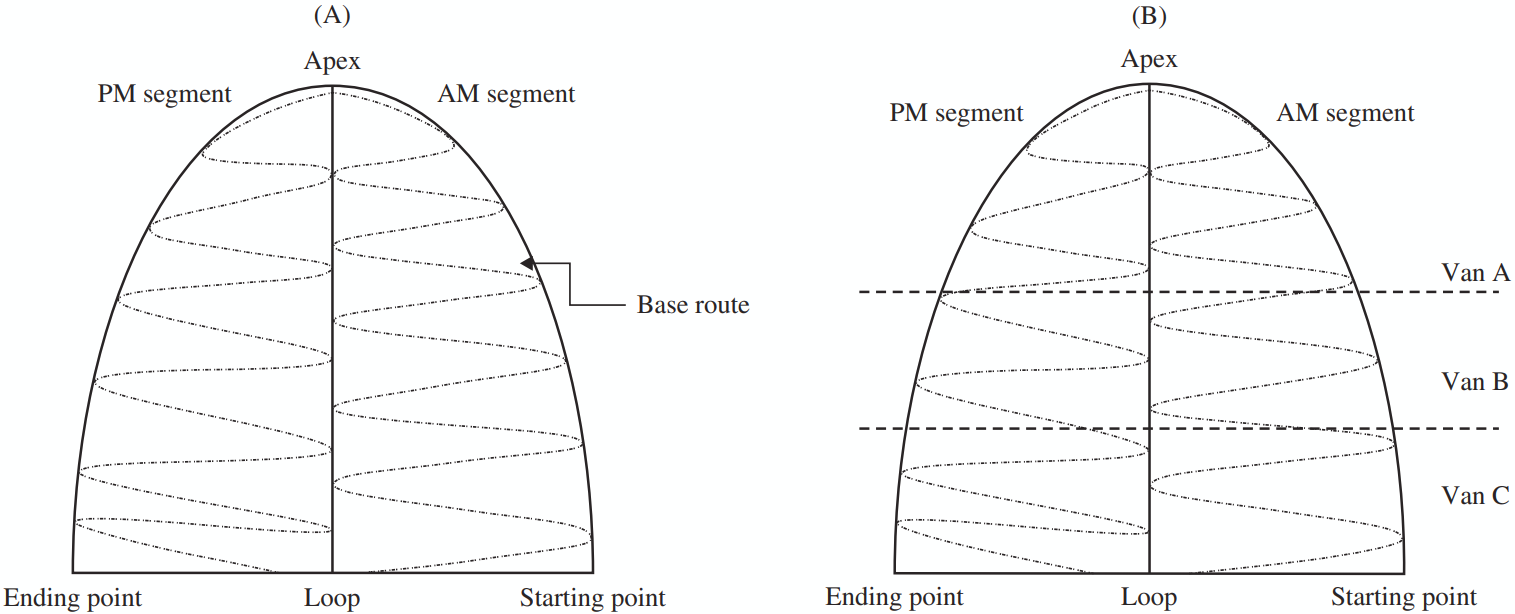
\includegraphics[width=0.8\textwidth]{../img/holland.png}
    \caption{Ruta base de un \emph{loop}: segmentos AM y PM unidos en un ápice y asignados a tres furgonetas (Holland et al., 2017).}
    \label{fig:holland}
\end{figure}

% =====================================================================
\section{Funcionamiento y técnicas de optimización}
% =====================================================================
\subsection{Funcionamiento general}
La carga de las furgonetas dura unas cuatro horas cada mañana. Durante ese lapso, ORION recopila cada minuto los paquetes cargados en cada vehículo y calcula una ruta optimizada \emph{desde cero}, ignorando la anterior, de modo que siempre exista una solución actualizada para planificadores y conductores \parencite{holland2017}. El conductor recibe la secuencia en su dispositivo portátil y puede preverla en quioscos del centro. La infraestructura descrita soporta 30\,000 optimizaciones de ruta por minuto, con matrices de tiempo y distancia calculadas por servidores dedicados, y las correcciones de mapas se propagan en unos 15 segundos \parencite{holland2017}. Con UPSNav (2019) se añadieron indicaciones giro a giro y, con \emph{Dynamic Optimization} (2020), ORION recalcula rutas durante la jornada según tráfico, recogidas y cambios en las entregas \parencite{ups2020}.

\subsection{Generación y optimización de rutas}
UPS probó primero una formulación entera del TSPTW y la descartó porque tardaba demasiado; tampoco halló algoritmos públicos, exactos o heurísticos, que cumplieran su requisito de velocidad: según sus cálculos, un minuto improductivo diario por conductor costaría 15 millones de dólares al año \parencite{holland2017}. Por eso desarrolló una metaheurística basada en búsqueda local. Los autores indican que su rutina contiene variantes de la heurística $k$-opt de Lin--Kernighan \parencite{lin1973}, búsqueda adaptativa de vecindad grande con vecindad de longitud variable \parencite{ropke2006}, relajación lagrangiana \parencite{lemarechal2001} y recocido simulado \parencite{ingber1993}, todas modificadas para respetar restricciones adicionales, como grupos de paradas con orden fijo. El detalle del algoritmo se mantiene como secreto industrial.

\subsection{Restricciones operativas documentadas}
\begin{itemize}
  \item \textbf{Ventanas de tiempo:} se tratan como restricciones blandas con penalización por retraso; el planificador puede definir un margen de seguridad que se aplica a las ventanas, por ejemplo en rutas con tráfico denso.
  \item \textbf{Consistencia:} cotas inferior y superior para la posición de cada cliente, deducidas del historial de entregas y de la ruta base, también como restricciones blandas. En temporada navideña, con las furgonetas muy cargadas, la ruta puede necesitar seguir más de cerca la ruta base.
  \item \textbf{Seguridad:} penalización de giros a la izquierda y de recorridos en zigzag sobre calles transitadas.
  \item \textbf{Prácticas operativas:} entregas comerciales temprano y recogidas al final del día.
  \item \textbf{Tráfico:} los tiempos de viaje provienen de mapas ajustados con datos GPS; la reacción al tráfico en vivo se incorporó con la versión dinámica \parencite{ups2020}.
  \item \textbf{Capacidad del vehículo:} en la formulación publicada no aparece como restricción del modelo de secuenciación, porque la asignación de paquetes a furgonetas se resuelve aparte.
\end{itemize}

\subsection{Mecanismos confirmados y alternativas teóricas}
La Tabla~\ref{tab:tecnicas} separa lo que las fuentes atribuyen a ORION de técnicas que el curso estudia pero que no están documentadas para este sistema.

\begin{table}[ht]
\centering\small
\caption{Técnicas confirmadas para ORION y alternativas solo teóricas}
\label{tab:tecnicas}
\begin{tabularx}{\textwidth}{@{}>{\raggedright\arraybackslash}p{4.5cm} >{\raggedright\arraybackslash}p{3.0cm} X@{}}
\toprule
Técnica & Estado & Observación \\
\midrule
Búsqueda local con variantes de Lin--Kernighan $k$-opt & Confirmada \parencite{holland2017} & Modificada para restricciones propias \\
Búsqueda de vecindad grande adaptativa & Confirmada \parencite{holland2017} & Con vecindad de longitud variable \\
Relajación lagrangiana & Confirmada \parencite{holland2017} & Rol exacto no detallado \\
Recocido simulado & Confirmada \parencite{holland2017} & Metaheurística estocástica \\
IA y aprendizaje automático & Declarada por UPS \parencite{ups2020} & Sin detalle técnico público \\
Modelo entero exacto (TSPTW) & Probada y descartada \parencite{holland2017} & Tiempo de solución excesivo \\
Programación dinámica de Held--Karp \parencite{held1962} & Alternativa teórica & No documentada en ORION \\
Búsqueda aleatoria Monte Carlo pura & Alternativa teórica & No hay evidencia de su uso \\
\bottomrule
\end{tabularx}
\end{table}

Esta clasificación conecta con el laboratorio: el recocido simulado es una búsqueda estocástica guiada, mientras que la búsqueda Monte Carlo pura muestrea soluciones al azar sin aprovechar la estructura del problema. El primer enfoque forma parte de lo documentado para ORION; el segundo, no.

% =====================================================================
\section{Magnitud del problema en la práctica}
% =====================================================================
\subsection{Paradas por conductor}
La cifra de paradas varía según la fuente (Tabla~\ref{tab:paradas}). Las diferencias obedecen a que corresponden a años distintos, a que unas son rangos y otras promedios, y a que una parada (cliente) puede incluir varios paquetes. En 2016 UPS entregaba en promedio más de 16 millones de paquetes diarios en EE.\,UU. con 55 000 conductores \parencite{holland2017}, lo que implica más de 290 paquetes por conductor (cálculo propio), es decir, aproximadamente dos paquetes por parada. En temporada alta el volumen puede duplicarse.

\begin{table}[ht]
\centering\small
\caption{Paradas diarias por conductor según distintas fuentes}
\label{tab:paradas}
\begin{tabularx}{\textwidth}{@{}l l X@{}}
\toprule
Valor reportado & Año & Fuente y naturaleza \\
\midrule
$\approx 120$ paradas & 2016 & \textcite{clevenger2016}: ruta típica \\
140--160 clientes (paradas) & 2016--2017 & \textcite{holland2017}: rango por conductor \\
135 paradas & 2020 & \textcite{ups2020}: promedio de ``muchos'' conductores \\
\bottomrule
\end{tabularx}
\end{table}

\subsection{Conductores y rutas}
\textcite{holland2017} reportan 55 000 conductores en EE.\,UU. y unos 1\,400 centros de paquetes. UPS informa después más de 66 000 rutas en Estados Unidos, Canadá y Europa \parencite{ups2020}. La Figura~\ref{fig:conductores} muestra el crecimiento de conductores que usaron ORION entre 2008 y 2016, según los datos del artículo; el valor de 2016 corresponde al despliegue completo previsto al redactarlo.

\begin{figure}[ht]
\centering
\begin{tikzpicture}
\begin{axis}[
  ybar, width=0.9\textwidth, height=6cm, bar width=14pt,
  symbolic x coords={2008,2009,2010,2011,2012,2013,2014,2015,2016},
  xtick=data, ymin=0, ymax=62000,
  ylabel={Conductores}, xlabel={Año},
  y tick label style={/pgf/number format/fixed, /pgf/number format/1000 sep={\,}},
  nodes near coords, nodes near coords align={vertical},
  every node near coord/.append style={font=\scriptsize, /pgf/number format/fixed, /pgf/number format/1000 sep={\,}},
  enlarge x limits=0.08
]
\addplot coordinates {(2008,21) (2009,68) (2010,268) (2011,268) (2012,1697) (2013,7150) (2014,20094) (2015,38456) (2016,55000)};
\end{axis}
\end{tikzpicture}
\caption{Conductores de EE.\,UU. que usaron ORION por año. Elaboración propia con datos de \textcite{holland2017}.}
\label{fig:conductores}
\end{figure}

\subsection{Escala geográfica y operativa}
ORION opera en los centros de paquetes de EE.\,UU. y, según UPS, también en Canadá y Europa \parencite{ups2020}. La infraestructura debe cubrir distintos husos horarios: una capacidad de 30\,000 rutas por minuto alcanza para los 55 000 conductores porque la carga de furgonetas se escalona entre costa y costa \parencite{holland2017}.

\subsection{Comparación con el TSP académico y fuerza bruta}
El ejemplo del laboratorio, con 5 ciudades y origen fijo, implica $4!=24$ recorridos, que se enumeran al instante. Para una ruta de UPS con $n$ paradas y un depósito fijo hay $n!$ secuencias posibles. La Tabla~\ref{tab:fuerzabruta} muestra su magnitud, suponiendo, de forma optimista, que se evalúan $10^{9}$ secuencias por segundo (cálculo propio).

\begin{table}[ht]
\centering\small
\caption{Crecimiento de las secuencias posibles de una ruta}
\label{tab:fuerzabruta}
\begin{tabular}{@{}r r r@{}}
\toprule
Paradas $n$ & Secuencias $n!$ & Tiempo a $10^{9}$ seq/s \\
\midrule
4 (ejemplo de 5 ciudades) & $24$ & instantáneo \\
10 & $3{,}6\times10^{6}$ & 3,6 ms \\
20 & $2{,}4\times10^{18}$ & $\approx 77$ años \\
120 & $6{,}7\times10^{198}$ & $\approx 10^{182}$ años \\
135 & $2{,}7\times10^{230}$ & $\approx 10^{214}$ años \\
150 & $5{,}7\times10^{262}$ & $\approx 10^{246}$ años \\
\bottomrule
\end{tabular}
\end{table}

Con 120 paradas, $n!$ supera por mucho cualquier cantidad física razonable, en línea con la observación cualitativa de \textcite{clevenger2016} de que las secuencias exceden los nanosegundos que lleva existiendo la Tierra. Tampoco basta una técnica exacta mejor que la fuerza bruta: la programación dinámica de Held--Karp \parencite{held1962} requiere del orden de $n^2 2^n$ operaciones, unas $10^{49{,}5}$ para $n=150$ (cálculo propio). Los solucionadores exactos modernos \parencite{applegate2006} resuelven instancias grandes de TSP puro, pero UPS necesita resolver unas 55 000 rutas con ventanas y consistencia en minutos y repetidamente, de ahí el uso de heurísticas.

% =====================================================================
\section{Resultados y beneficios}
% =====================================================================
La Tabla~\ref{tab:resultados} reúne las cifras verificables, indicando su naturaleza, porque algunas son proyecciones y otras son resultados reportados.

\begin{table}[ht]
\centering\small
\caption{Resultados reportados de ORION}
\label{tab:resultados}
\begin{tabularx}{\textwidth}{@{}>{\raggedright\arraybackslash}p{3.3cm} X >{\raggedright\arraybackslash}p{3.6cm}@{}}
\toprule
Indicador & Valor & Naturaleza y fuente \\
\midrule
Distancia recorrida & $\approx 100$ millones de millas por año ($\approx 161$ millones de km) & Proyección a despliegue completo \parencite{holland2017}; reportado por UPS \parencite{ups2020} \\
Combustible & $\approx 10$ millones de galones por año ($\approx 38$ millones de litros) & Igual que el anterior \\
Emisiones de CO$_2$ & $\approx 100\,000$ toneladas métricas por año & Proyección \parencite{holland2017} \\
Ahorro económico & 300--400 millones de dólares por año & Proyección a despliegue completo \parencite{holland2017} \\
Ahorro acumulado & 320 millones de dólares hasta diciembre de 2015, con costo de 295 millones & Reportado y verificado por un grupo interno de UPS \parencite{holland2017} \\
Millas por conductor & 8 por conductor (ORION original) y 2--4 con la versión dinámica & Declaración ejecutiva \parencite{leonard2021} \\
Valor de un minuto o una milla & 14,6 millones de dólares por minuto; 50 millones por milla por conductor al día & \textcite{clevenger2016} \\
\bottomrule
\end{tabularx}
\end{table}

Algunas diferencias merecen explicación. Un comunicado de 2015 también proyectaba 100 millones de millas, 10 millones de galones y más de 300 millones de dólares anuales \parencite{ups2015}. El valor de un minuto improductivo es de 15 millones de dólares en \textcite{holland2017} y de 14,6 millones en \textcite{clevenger2016}; se trata de redondeos de una misma magnitud. Como comprobación de consistencia, 100 millones de millas entre 55 000 conductores y 250 días laborables equivalen a unas 7,3 millas diarias por conductor (cálculo propio), cifra cercana a las 8 millas declaradas.

Los resultados también deben leerse con cautela: provienen de UPS o de entrevistas con sus directivos, se comparan con la práctica previa basada en el criterio del conductor, y los 85 millones de millas atribuidos a las PFT anteriores a 2011 \parencite{holland2017} son un beneficio distinto que no debe sumarse al de ORION. Los autores reconocen además que algunos conductores aún superan a ORION en ciertas rutas. Entre los beneficios no financieros se mencionan la posibilidad de ofrecer entregas con ventana horaria como servicio de pago, el uso del sistema para fijar precios y una conducción más segura al liberar al conductor de la planificación.

\begin{figure}[H]
    \centering
    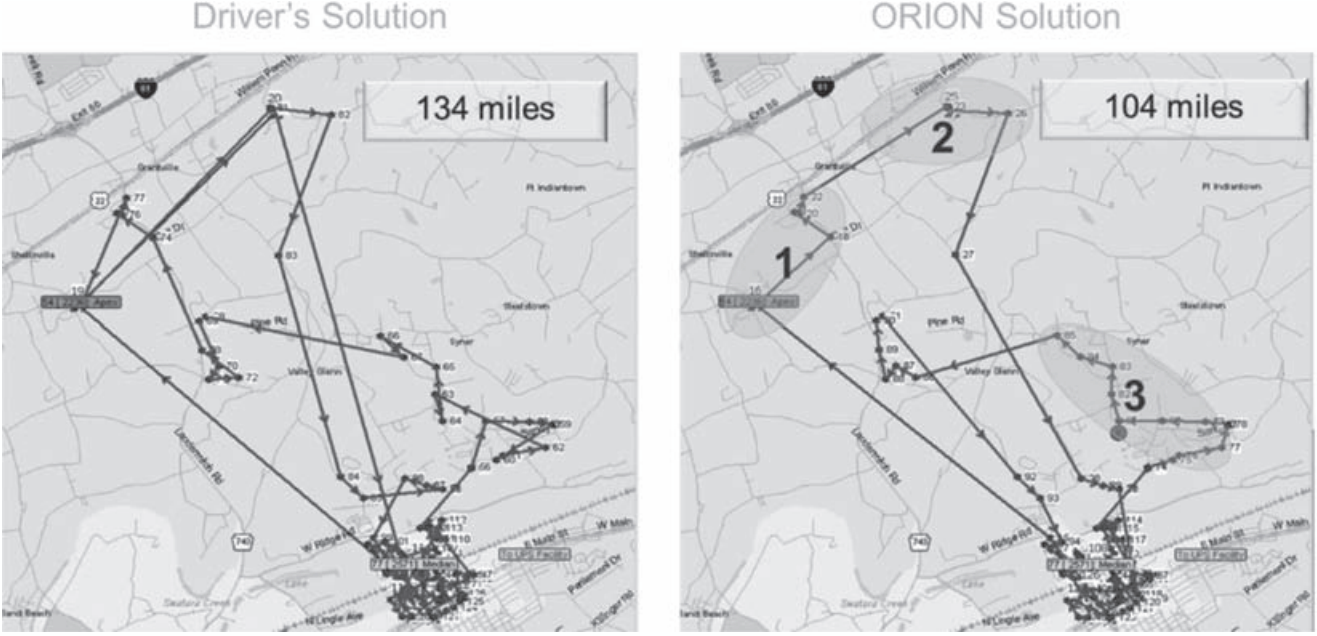
\includegraphics[width=0.8\textwidth]{../img/driver_orion.png}
    \caption{Comparación de la ruta del conductor y la de ORION; esta última visita dos áreas una sola vez y evita 30 millas (Holland et al., 2017).}
    \label{fig:comparacion}
\end{figure}

\section{Conclusiones}
% =====================================================================
El caso ORION conecta de forma directa con los conceptos del laboratorio. Cada conductor enfrenta un problema de secuenciación equivalente a un TSP con ventanas de tiempo sobre 120 a 160 paradas, un tamaño para el cual enumerar permutaciones (como en el ejemplo de 5 ciudades) es imposible, pues $n!$ supera $10^{198}$ ya con 120 paradas. A esto se suma que el TSP es NP-difícil, y su variante con ventanas de tiempo lo es también.

La enseñanza principal es el papel de las heurísticas. UPS comprobó que un modelo entero exacto era demasiado lento y que ninguna heurística pública cumplía su requisito de velocidad, así que construyó una metaheurística propia a partir de componentes conocidos de búsqueda local y recocido simulado. El desempeño no se midió solo por el costo de la función objetivo: la regularidad día a día, la seguridad y la aceptación de los conductores fueron determinantes, y su primer intento falló, entre otras razones, por ignorar la consistencia y por la mala calidad de los mapas \parencite{holland2017}.

Esto muestra las limitaciones de los modelos clásicos. El TSP básico supone distancias fijas y conocidas, un solo objetivo y ninguna restricción práctica; el problema real exige ventanas horarias, consistencia, asimetría de costos, información que llega tarde y reoptimización continua. Por eso el TSP es un punto de partida y no una descripción completa de ORION.

Finalmente, el caso ilustra el valor económico de la optimización algorítmica: según UPS, un solo minuto o una sola milla diaria por conductor tienen un valor de decenas de millones de dólares anuales. Conviene recordar los límites de este informe: las cifras de resultados provienen de la propia empresa, las más recientes encontradas datan de 2020--2021 y el algoritmo exacto no es público.

% =====================================================================
% REFERENCIAS
% =====================================================================
\printbibliography[title={Referencias bibliográficas}]

\end{document}